\documentclass[a4paper]{article}
\usepackage[UTF8]{ctex}
\usepackage[a4paper,margin=1in]{geometry}
\usepackage{graphicx}
\usepackage{float}
\usepackage{listings}
\usepackage{booktabs}
\usepackage{hyperref}
\usepackage{fancyhdr}
\usepackage{lastpage}
\usepackage{color}
\usepackage{xcolor}
\usepackage{indentfirst}
\setlength{\parindent}{2em}
\usepackage{zhnumber}
\usepackage[dvipsnames]{xcolor}
\usepackage{amsmath}
\usepackage{tikz}
\usetikzlibrary{shapes,arrows,positioning}

% ===== 个人信息与实验信息配置 =====
\newcommand{\projname}{ROSE——编译原理逆向工程工具}
\newcommand{\reporttitle}{实验四-设计文档}
\newcommand{\stuno}{23336179}
\newcommand{\authorname}{马福泉}
\newcommand{\major}{计算机科学与技术}
\newcommand{\adviser}{李文军}
\newcommand{\startdate}{2026年6月}
\newcommand{\labenddate}{2026年6月}
\newcommand{\labroom}{B203}

% ===== 页眉页脚设置 =====
\pagestyle{fancy}
\fancyhf{}
\fancyhead[L]{\kaishu \projname}
\fancyhead[C]{\kaishu \reporttitle}
\fancyhead[R]{\kaishu \authorname}
\fancyfoot[C]{第 \thepage 页，共 \pageref{LastPage} 页}
\renewcommand{\headrulewidth}{0.4pt}
\renewcommand{\footrulewidth}{0pt}

% ===== 代码高亮配置 =====
\definecolor{NavyBlue}{RGB}{0,0,128}
\definecolor{codegreen}{RGB}{0,128,0}
\definecolor{codegray}{RGB}{128,128,128}
\definecolor{codepurple}{RGB}{128,0,128}
\definecolor{backcolour}{RGB}{245,245,245}

\lstset{
    language=Java,
    basicstyle=\ttfamily\small,
    commentstyle=\color{codegreen}\itshape,
    keywordstyle=\color{NavyBlue}\bfseries,
    stringstyle=\color{codepurple},
    numberstyle=\tiny\color{codegray},
    backgroundcolor=\color{backcolour},
    breaklines=true,
    frame=single,
    numbers=left,
    tabsize=4,
    showstringspaces=false,
    captionpos=b,
    escapeinside={\%}{\%},
    morekeywords={enum,record}
}

\begin{document}

% ==================== 封面 ====================
\begin{titlepage}
    \centering
    
    
\includegraphics[width=10cm]{img/SYSULogo.png}

    \vspace{1em}
    {\Large \kaishu \projname \par}
    \vspace{3em}

    {\fontsize{36pt}{40pt}\kaishu \selectfont \boldmath \reporttitle\par}
    \vspace{2em}
    \vspace*{\fill}

    \begin{center}
    {\Large
    \makebox[5em][s]{学号}:\underline{\makebox[15em][c]{\kaishu \stuno}}\\[1em]
    \makebox[5em][s]{姓名}:\underline{\makebox[15em][c]{\kaishu \authorname}}\\[1em]
    \makebox[5em][s]{专业}:\underline{\makebox[15em][c]{\kaishu \major}}\\[1em]
    \makebox[5em][s]{指导教师}:\underline{\makebox[15em][c]{\kaishu \adviser}}\\[1em]
    \makebox[5em][s]{起始日期}:\underline{\makebox[15em][c]{\kaishu \startdate}}\\[1em]
    \makebox[5em][s]{结束日期}:\underline{\makebox[15em][c]{\kaishu \labenddate}}\\[1em]
    \makebox[5em][s]{实验地点}:\underline{\makebox[15em][c]{\kaishu \labroom}}
    }
    \end{center}

    \vspace*{\fill}
\end{titlepage}

% ==================== 目录 ====================
\tableofcontents
\newpage

% ==================== 正文 ====================

\section{实验简述}

本项目 ROSE 是一个编译原理逆向工程工具，旨在对 Oberon-0 语言源程序进行词法分析、语法分析、
语义分析，并自动生成流程图和调用关系图。本实验为第四阶段——手工编写递归下降预测分析程序，
替代前序实验中由工具（JavaCUP）自动生成的 LALR 语法分析器。在解析过程中，使用 ROSE 工具
集的 \texttt{flowchart.*} API 构建控制流模型，最终以可视化流程图形式呈现每个过程的
语句级控制流结构。

本实验的核心挑战在于：(1) 精确理解 Oberon-0 文法中隐含的左递归结构（主要出现在表达式层级），
并在递归下降代码中以 while 循环实现闭包消除；(2) 设计每个非终结符的解析方法签名——继承属性
作为方法参数传入，综合属性作为返回值传出；(3) 在解析过程中同步构造 \texttt{flowchart.*}
图模型节点并建立它们之间的嵌套关系。

\section{Oberon-0 语言的 LL(1) 改造与翻译模式}

\subsection{左递归消除策略}

Oberon-0 的 EBNF 文法在表达式层级隐含左递归，例如：

\begin{verbatim}
Expression       = SimpleExpression [Relation SimpleExpression] .
SimpleExpression = ["+"|"-"] Term {AddOperator Term} .
Term             = Factor {MulOperator Factor} .
\end{verbatim}

原始文法中 \texttt{SimpleExpression} 和 \texttt{Term} 的迭代结构（花括号闭包）通过 EBNF
运算符 \texttt{\{\ \}} 隐式表达了左递归。在手工递归下降代码中，这些闭包直接转换为 \texttt{while}
循环，无需显式改写文法：

\begin{itemize}
    \item \texttt{\{AddOperator Term\}} → \texttt{while (check(PLUS) || check(MINUS) || check(OR)) \{ ... \}}
    \item \texttt{\{MulOperator Factor\}} → \texttt{while (check(STAR) || check(DIV) || check(MOD) || check(AND)) \{ ... \}}
\end{itemize}

声明序列的递归同样通过 while 循环表达：

\begin{itemize}
    \item \texttt{DeclarationSequence = \{ CONST ... | TYPE ... | VAR ... | ProcDecl ... \}}
          → \texttt{while (CONST | TYPE | VAR | PROCEDURE) \{ switch(lookahead) ... \}}
\end{itemize}

\subsection{翻译模式伪代码}

以下以带语义动作的翻译模式展示核心解析逻辑（用 Java 风格注释标注语义动作位置）：

{\small
\begin{verbatim}
/* Module */
parseModule():
    match(MODULE); match(IDENT); match(SEMI);
    module = new FlowchartModule(id);
    parseDeclarationSequence();
    if check(BEGIN):
        match(BEGIN);
        mainProc = module.add(moduleName + "$body");
        parseStatementSequence(mainProc);
    match(END); match(IDENT); match(DOT);
    return module;

/* ProcedureDeclaration */
parseProcedureDeclaration():
    match(PROCEDURE); match(IDENT);
    proc = module.add(procName);          // 语义动作: 创建 Procedure
    if check(LPAREN): parseFormalParameters();
    match(SEMI);
    parseDeclarationSequence();            // 局部声明
    if check(BEGIN):
        match(BEGIN);
        parseStatementSequence(proc);     // 过程体
    match(END); match(IDENT);

/* StatementSequence */
parseStatementSequence(target):           // target = Procedure | StatementSequence
    stmt = parseStatement();
    if stmt != null: target.add(stmt);    // 语义动作: 添加语句节点
    while check(SEMI):
        match(SEMI);
        stmt = parseStatement();
        if stmt != null: target.add(stmt);

/* IfStatement */
parseIfStatement():
    match(IF); cond = parseExpression(); match(THEN);
    ifStmt = new IfStatement(cond);        // 语义动作: 创建 If 节点
    parseStatementSequence(ifStmt.getTrueBody());   // True 分支
    while check(ELSIF):
        match(ELSIF);
        nestedIf = new IfStatement(cond2); // 嵌套 If 模拟 ELSIF
        parseStatementSequence(nestedIf.getTrueBody());
        ifStmt.getFalseBody().add(nestedIf);
        ifStmt = nestedIf;
    if check(ELSE):
        match(ELSE);
        parseStatementSequence(ifStmt.getFalseBody());  // False 分支
    match(END);
    return ifStmt;

/* WhileStatement */
parseWhileStatement():
    match(WHILE); cond = parseExpression(); match(DO);
    whileStmt = new WhileStatement(cond);  // 语义动作: 创建 While 节点
    parseStatementSequence(whileStmt.getLoopBody());    // 循环体
    match(END);
    return whileStmt;

/* Expression (含闭包消除) */
parseExpression():
    left = parseSimpleExpression();
    if check(REL_OP):                     // {= | # | < | <= | > | >=}
        op = getRelationOp();
        right = parseSimpleExpression();
        left = left + op + right;         // 综合属性: 表达式字符串
    return left;

parseSimpleExpression():
    sign = (check(PLUS) | check(MINUS)) ? match() : "";
    result = sign + parseTerm();
    while check(PLUS) | check(MINUS) | check(OR):  // {AddOperator Term}
        op = match(); result = result + op + parseTerm();
    return result;

parseTerm():
    result = parseFactor();
    while check(STAR) | check(DIV) | check(MOD) | check(AND):  // {MulOperator Factor}
        op = match(); result = result + op + parseFactor();
    return result;
\end{verbatim}
}

\subsection{继承属性与综合属性的传递}

在递归下降翻译模式中，属性传递极其自然：

\begin{itemize}
    \item \textbf{继承属性}（从上文传入下文的上下文信息）通过\textbf{方法参数}传递。
          例如 \texttt{parseStatementSequence(target)} 中 \texttt{target} 参数告知
          解析过程中将生成的语句节点添加到哪个容器（Procedure 或 IfStatement 的 True/False 分支）。
    \item \textbf{综合属性}（从子节点汇总到父节点的计算结果）通过\textbf{方法返回值}传递。
          例如 \texttt{parseExpression()} 返回表达式的字符串表示，\texttt{parseIfStatement()}
          返回构建好的 \texttt{IfStatement} 节点。
    \item \textbf{局部变量}保存中间结果（如表达式累积过程中的运算符和操作数拼接），避免引入
          不必要的继承属性传播。
\end{itemize}

这种属性传递模式与 LALR 分析器形成鲜明对比——LALR 的继承属性只能通过全局栈或
特殊占位符（如 CUP 中的 \texttt{RESULT} 隐式变量）传递，而递归下降的面向对象方法签名
提供了对属性流的全透明控制。

\section{语法分析讨论：自顶向下 vs. 自底向上}

\subsection{递归下降 (LL) 与 LR/LALR 的综合对比}

表~\ref{tab:ll-lr} 从多个维度系统对比递归下降 LL 分析与 LR/LALR 分析。

\begin{table}[H]
\centering
\caption{自顶向下 (递归下降 LL) 与自底向上 (LR/LALR) 语法分析综合对比}
\label{tab:ll-lr}
\begin{tabular}{@{}p{3cm}p{5.5cm}p{5.5cm}@{}}
\toprule
\textbf{维度} & \textbf{递归下降 (LL|自顶向下)} & \textbf{LR/LALR (自底向上)} \\
\midrule
实现方式 & 手工编写，每个非终结符一个方法 & 工具自动生成，基于分析表 \\
代码与文法的对应 & 与文法同构，直观映射 & 状态机驱动，不直观 \\
调试难度 & 极低——IDE 设断点、单步跟踪、观察调用栈 & 极高——依赖分析表和状态机，如黑盒操作 \\
文法限制 & 必须为 LL(1)，需消除左递归和左公因子 & 支持所有确定性上下文无关文法 \\
左递归处理 & 必须改写为迭代/右递归 & 原生支持，文法更自然 \\
语义动作表达 & 方法参数传递继承属性、返回值传递综合属性，极其自然 & 继承属性传递受限，常需全局栈或占位符 \\
错误恢复 & 恐慌模式（Panic-mode）同步集合，易于操作 & \texttt{error} 伪非终结符，需巧妙设计 \\
分析速度 & 大量函数调用，较慢 & 表驱动，稳定 $O(n)$，极快 \\
分析表大小 & 若改造为表驱动 LL(1)，表远小于 LR 表 & LR 表通常庞大（本实验三为 182 状态） \\
通用性 & 受限，不能处理二义性文法 & 可处理更广泛的文法类 \\
可伸缩性 & 适合教学语言和小型 DSL & 适合工业级通用编程语言 \\
\bottomrule
\end{tabular}
\end{table}

\subsection{各维度深度分析}

\textbf{(1) 简单性与调试}：递归下降的代码结构与 BNF 文法同构——\texttt{parseIfStatement}、
\texttt{parseWhileStatement}、\texttt{parseExpression} 等方法名直接对应非终结符，方法体
中的 \texttt{match()} 调用对应终结符消费，if/while 分支对应产生式选择。在 IDE 中可以在
任意方法调用处设断点，观察当前的向前看符号（\texttt{lookahead}）和解析状态，跟踪调用
栈即可回溯分析路径。相比之下，LR 分析器依赖编译时生成的状态转移表和运行时维护的状态栈，
代码与文法之间的映射被压缩为二维数组索引，调试几乎只能依赖推理和逐行的状态栈打印。

\textbf{(2) 通用性}：LR 族（包括 LALR）是处理能力最强的确定性语法分析技术，可以接受几乎
所有实际的编程语言文法。递归下降受限于 LL(1) 条件——每个产生式的 FIRST 集两两不相交，
且不含左递归。这就要求对文法进行预处理（消除左递归、提取左公因子），对复杂文法（如 C++
中歧义的嵌套模板声明 \texttt{vector<vector<int>>}）可能从根本上无法改写。

\textbf{(3) 语义动作表达}：这是递归下降的绝对优势领域。以 \texttt{parseStatementSequence(target)}
为例，\texttt{target} 参数直接携带了语句序列所属的容器引用——可以是过程的主体、IF 的 True
分支或 WHILE 的循环体，语义动作 \texttt{target.add(stmt)} 直接操作流程图节点，无需任何
中间数据结构。在 LALR 分析中，继承属性需要通过 \texttt{\$\$} 符号栈的返回值逐层上传，
或借助全局变量等受控副作用实现，极大地增加了代码的理解成本。

\textbf{(4) 出错恢复}：递归下降可以方便地实现恐慌模式错误恢复。当解析过程遇到意料之外的 Token
时，可以跳过输入 Token 直到遇到同步符号集合（如分号、END、右大括号等"恢复边界"），然后从对
应的非终结符方法重新开始解析。例如在 \texttt{parseStatementSequence} 中遇到语法错误后可以
调用 \texttt{skipTo(SEMI, END, ELSE)} 跳过错误输入段，然后继续解析后续语句——这在交互式
IDE 场景下可以实现单轮多错误报告。

\textbf{(5) 分析表大小与速度}：递归下降由于每个非终结符都是独立的方法调用，运行时开销主要
来自 Java 方法调用栈的开辟与恢复。LR 分析器将所有转移逻辑编码在单一的二维分析表中，循环
迭代 shift/reduce 而无函数调用开销，实测速度通常是递归下降的 2-5 倍。但若将递归下降改写
为表驱动 LL(1)，其分析表远小于 LR 表（LL(1) 表行数为非终结符数 $|N|$，LR 表行数为状态数
$|S|$，通常 $|S| \gg |N|$），内存占用更优。

\textbf{(6) 小结}：选择递归下降还是 LALR 本质上是选择"开发时的可控性"还是"运行时的
通用性与性能"。在本实验（Oberon-0 教学语言）的语境下，递归下降的简洁直观使其成为
最优选择；而在工业级编译器（GCC 使用手写递归下降，Clang 使用手写递归下降，javac 使用
手写递归下降——这恰说明工程中 LL 的实际应用比理论预测更广泛）中，手工递归下降因其
错误消息质量、语义动作灵活性和可调试性而占据主导地位。

\section{生成与编译结果}

\subsection{批处理脚本说明}

实验四提供三支批处理脚本：
\begin{itemize}
    \item \texttt{build.bat} —— 编译 OberonParser.java、OberonParserTest.java 及所有依赖
          （OberonScanner、Token、异常类），classpath 包含 \texttt{flowchart.jar} 和
          \texttt{jgraph.jar}。
    \item \texttt{run.bat} —— 运行递归下降解析器解析指定的 Oberon-0 源文件，成功解析后
          自动弹出流程图窗口。
    \item \texttt{test.bat} —— 运行单个变异测试用例。
    \item \texttt{gendoc.bat} —— 调用 \texttt{javadoc} 对 \texttt{src/} 下所有手写
          Java 源码（OberonParser.java、OberonParserTest.java、Token.java 及 5 个异常类）
          生成 HTML API 文档，输出至 \texttt{doc/} 目录。classpath 包含
          \texttt{flowchart.jar} 和 \texttt{jgraph.jar}。
\end{itemize}

\subsection{编译截图}

图~\ref{fig:build-ex4} 展示了 \texttt{build.bat} 的执行结果：
OberonParser.java（递归下降核心）、OberonParserTest.java（测试驱动）以及复用的
OberonScanner.java / Token.java / 5 个异常类全部编译通过。

\begin{figure}[H]
\centering
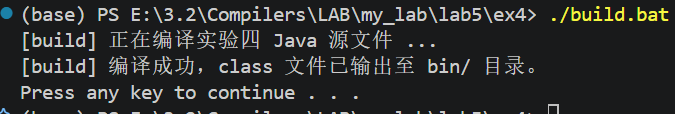
\includegraphics[width=0.9\textwidth]{img/build_ok.png}
\caption{build.bat 执行结果：递归下降解析器全部编译通过}
\label{fig:build-ex4}
\end{figure}

\subsection{运行截图}

图~\ref{fig:parse-ex4} 展示了 \texttt{run.bat} 解析 \texttt{StudentStats.obr} 的结果：
递归下降语法分析通过，弹出 Flowchart 可视化窗口，展示每个过程的控制流图（包括
CalcTotalAndAvg、ReadStudent、FindBestStudent、CheckAllPass、PrintStudent、PrintAll
六个过程的 While 循环和 IF/ELSIF/ELSE 分支结构）。

\begin{figure}[H]
\centering
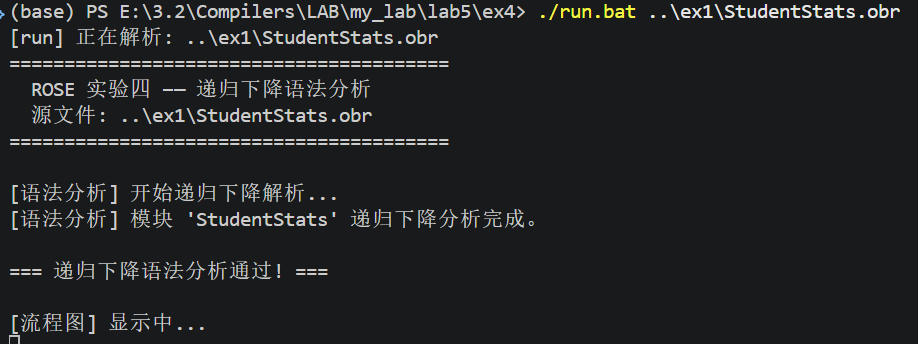
\includegraphics[width=0.9\textwidth]{img/parse_ok.png}
\caption{递归下降解析 StudentStats.obr —— 语法分析通过 + Flowchart 流程图}
\label{fig:parse-ex4}
\end{figure}

\section{语法分析与流程图生成运行结果}

\subsection{编译与解析测试}

图~\ref{fig:build-ex4-run} 与图~\ref{fig:parse-ex4-run} 展示了实验四 Java 源码的编译
与递归下降语法分析运行结果。所有源文件（OberonParser.java、OberonParserTest.java、
OberonScanner.java、Token.java 及 5 个异常类）均通过 javac 编译，随后对
\texttt{StudentStats.obr} 执行递归下降解析，解析成功并触发 Flowchart 流程图窗口弹出。

\begin{figure}[htbp]
    \centering
    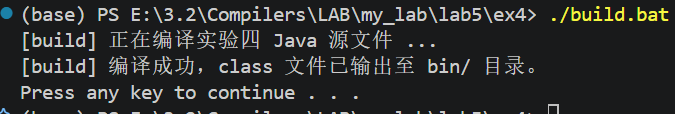
\includegraphics[width=0.8\textwidth]{img/build_ok.png}
    \caption{实验四 Java 源码编译成功}
    \label{fig:build-ex4-run}
\end{figure}

\begin{figure}[htbp]
    \centering
    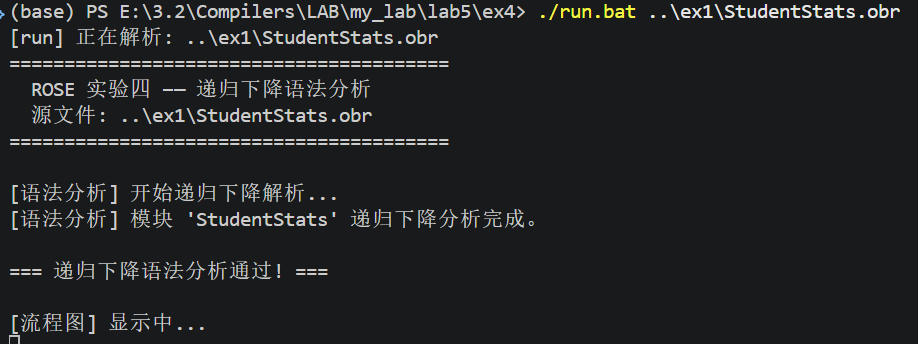
\includegraphics[width=0.8\textwidth]{img/parse_ok.png}
    \caption{递归下降语法分析通过并触发流程图绘制}
    \label{fig:parse-ex4-run}
\end{figure}

\subsection{核心流程图展示}

本节选取最具代表性的两张流程图进行展示：\texttt{CalcTotalAndAvg} 过程（包含 WHILE
循环和 IF 条件分支的嵌套结构）与 \texttt{StudentStats} 主程序体（展示模块入口到各
过程调用的顶层控制流）。

\begin{figure}[htbp]
    \centering
    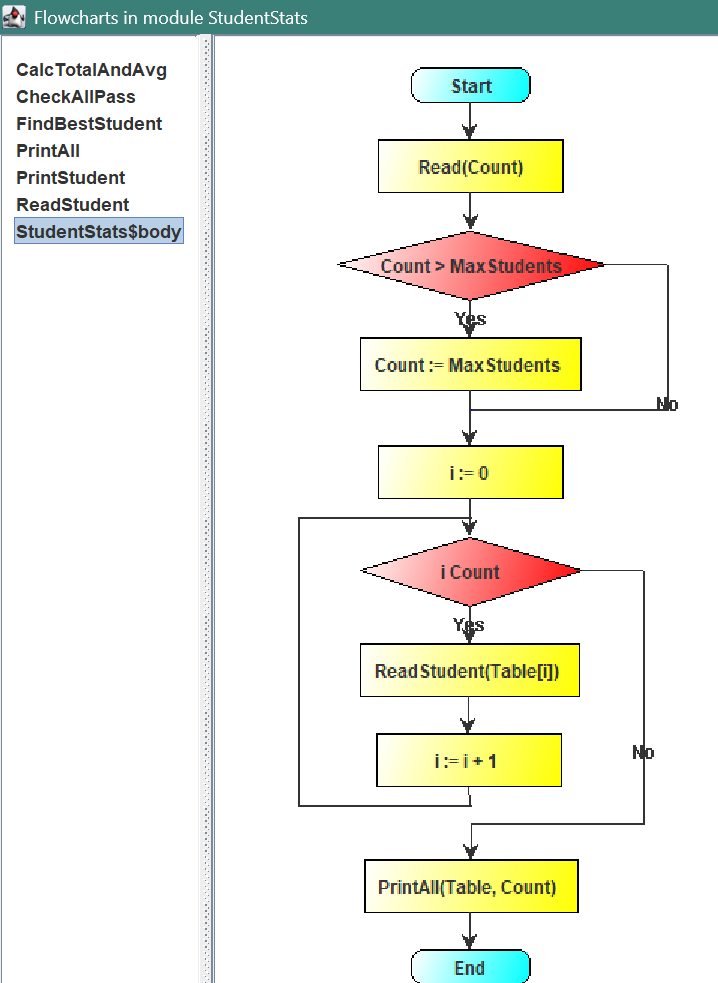
\includegraphics[width=0.5\textwidth]{img/stu.png}
    \caption{主程序 StudentStats 的流程图（含 BEGIN 语句体与过程调用序列）}
    \label{fig:flow-stu}
\end{figure}

\begin{figure}[htbp]
    \centering
    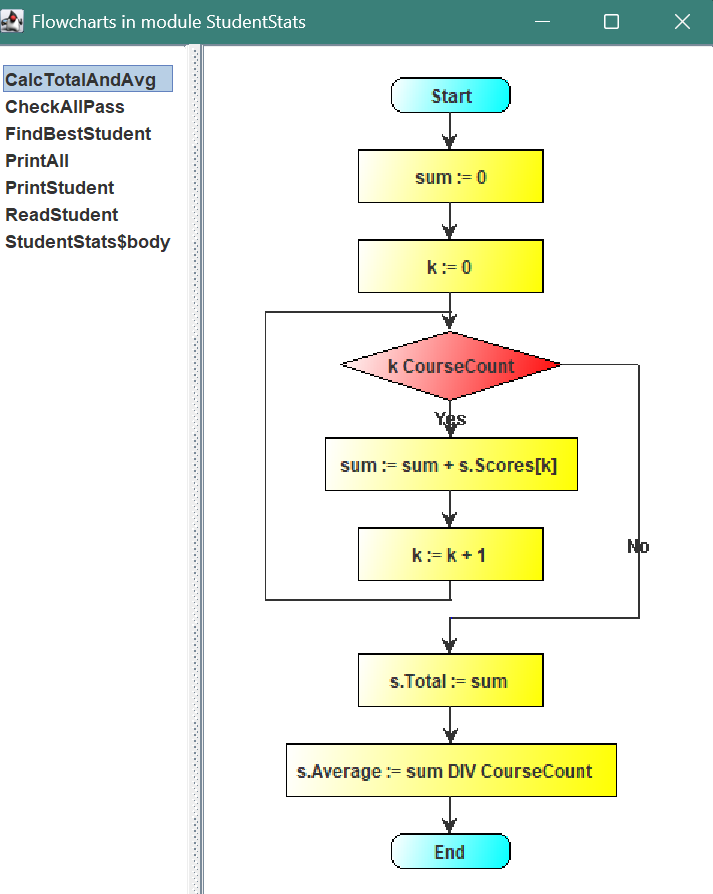
\includegraphics[width=0.5\textwidth]{img/calc.png}
    \caption{CalcTotalAndAvg 过程的流程图（含 WHILE 循环与 IF 条件分支）}
    \label{fig:flow-calc}
\end{figure}

\subsection{其他核心过程流程图}

以下展示 ReadStudent、PrintStudent、FindBestStudent、CheckAllPass 四个辅助过程的
流程图，完整覆盖了 Oberon-0 语言中 READ/WRITE 原语、WHILE 循环、IF/ELSIF/ELSE
多分支选择等核心控制结构的可视化表达。

\begin{figure}[htbp]
    \centering
    \begin{minipage}[t]{0.4\textwidth}
        \centering
        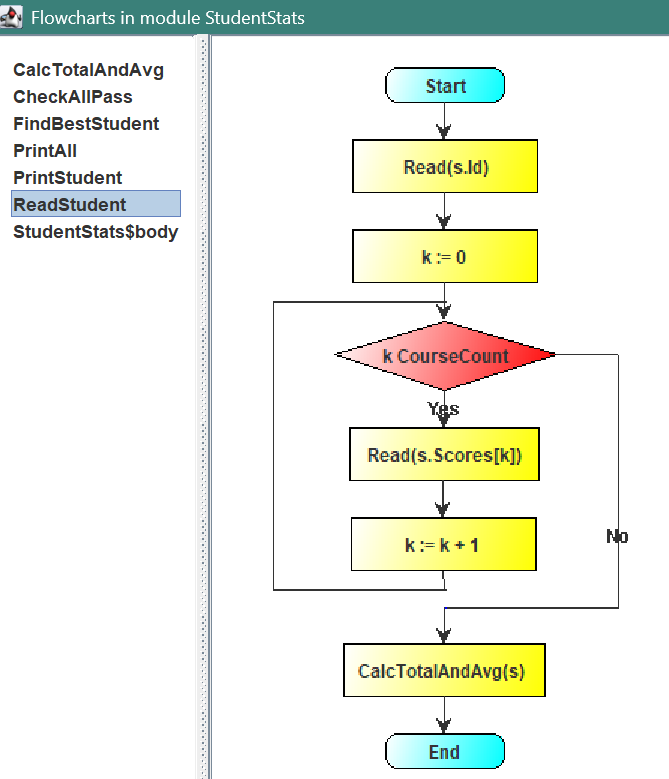
\includegraphics[width=\textwidth]{img/read_stu.png}
        \caption{ReadStudent 过程流程图}
        \label{fig:flow-read}
    \end{minipage}
    \hfill
    \begin{minipage}[t]{0.3\textwidth}
        \centering
        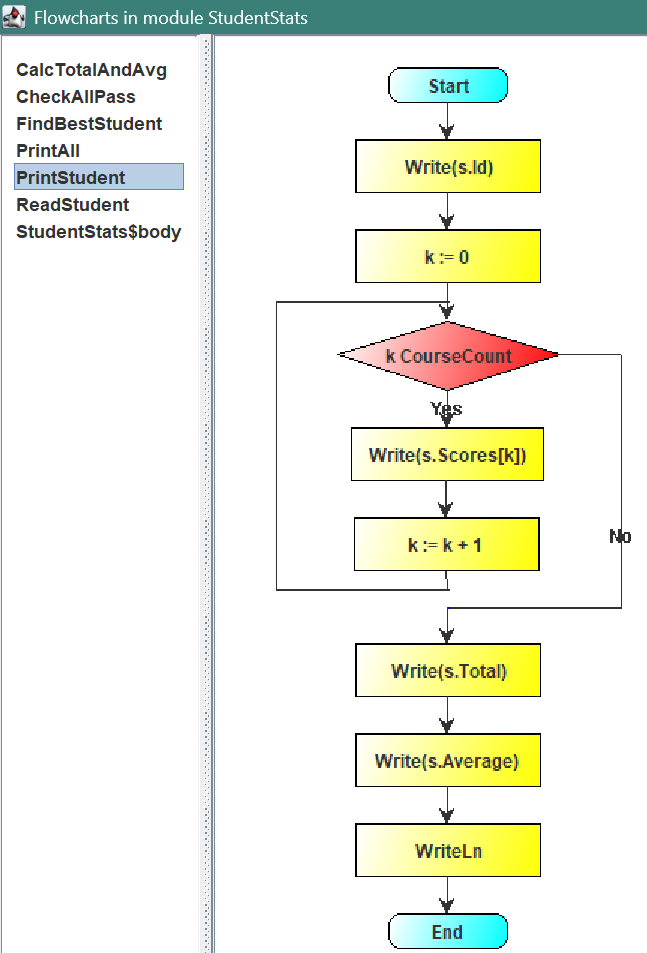
\includegraphics[width=\textwidth]{img/print_stu.png}
        \caption{PrintStudent 过程流程图}
        \label{fig:flow-print}
    \end{minipage}
\end{figure}

\begin{figure}[htbp]
    \centering
    \begin{minipage}[t]{0.35\textwidth}
        \centering
        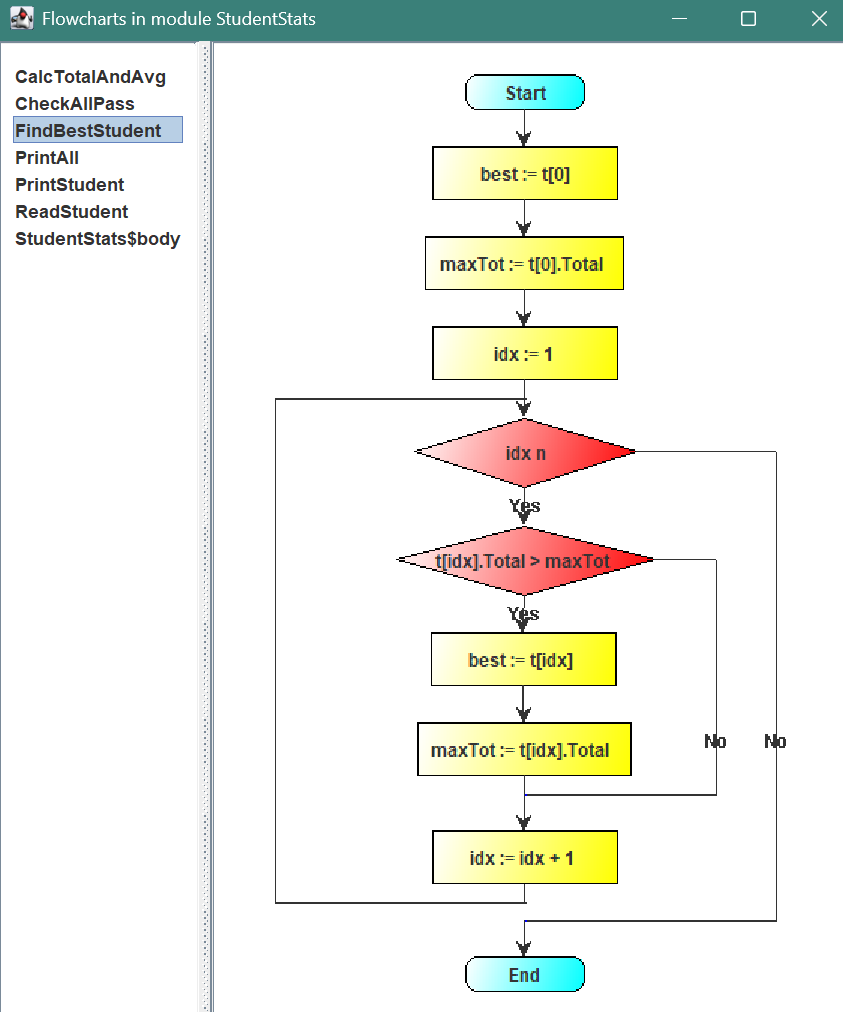
\includegraphics[width=\textwidth]{img/find.png}
        \caption{FindBestStudent 过程流程图}
        \label{fig:flow-find}
    \end{minipage}
    \hfill
    \begin{minipage}[t]{0.4\textwidth}
        \centering
        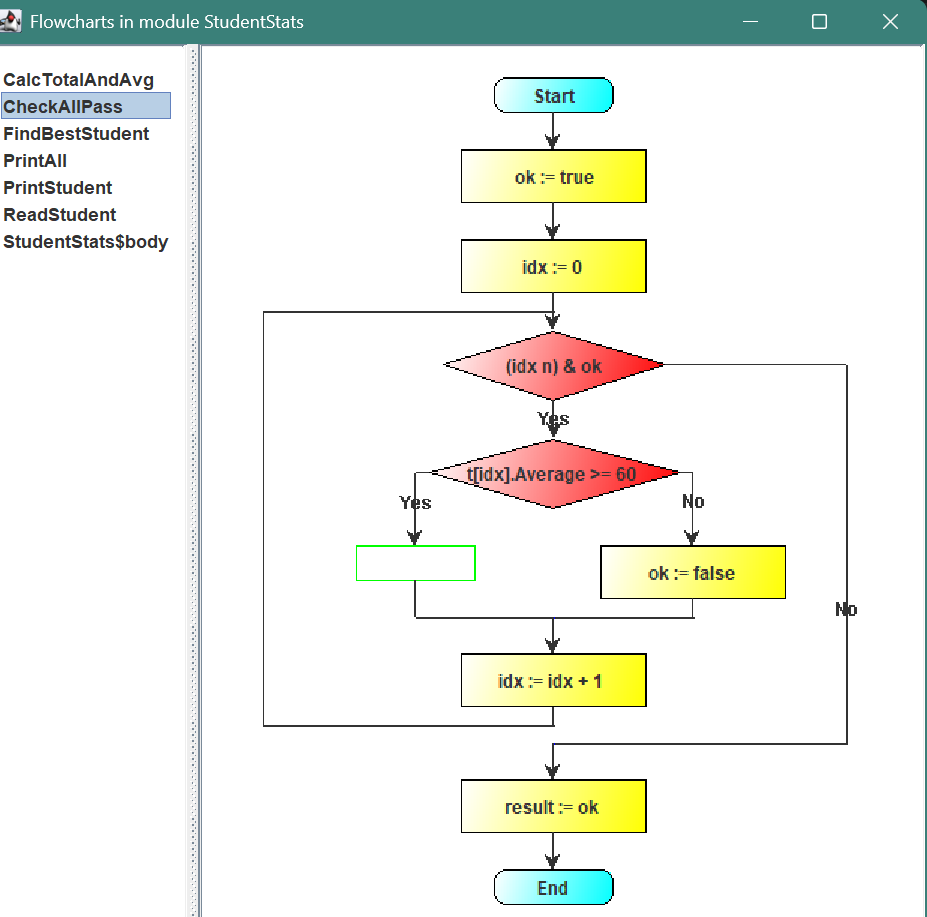
\includegraphics[width=\textwidth]{img/check.png}
        \caption{CheckAllPass 过程流程图}
        \label{fig:flow-check}
    \end{minipage}
\end{figure}

\subsection{长流程图并排展示 (PrintAll)}

由于 \texttt{PrintAll} 过程包含复杂的嵌套与顺序逻辑，流程图较长，此处采用并排方式展示
其上下两部分：

\begin{figure}[htbp]
    \centering
    \begin{minipage}[t]{0.5\textwidth}
        \centering
        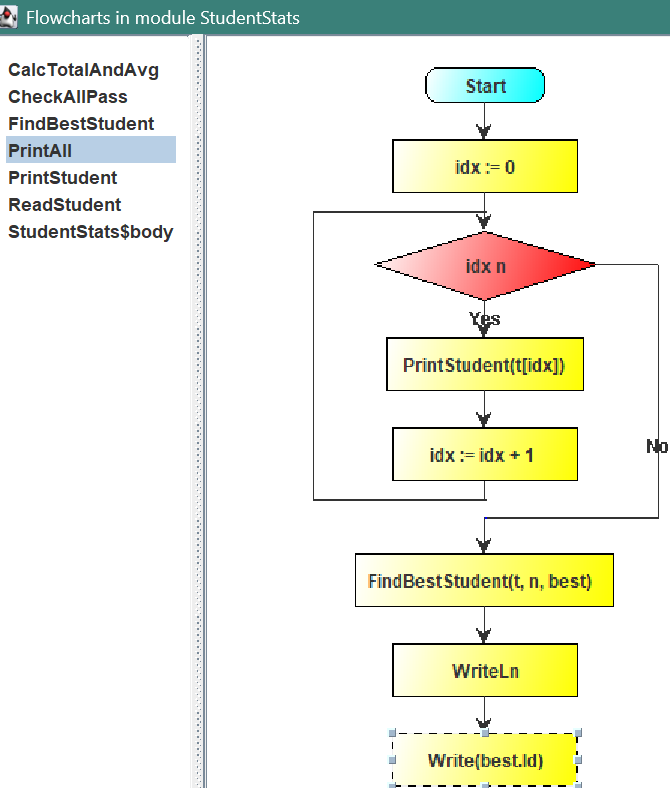
\includegraphics[width=\textwidth]{img/print_all1.png}
        \caption{PrintAll 流程图 (上半部分)}
        \label{fig:flow-printall1}
    \end{minipage}
    \hfill
    \begin{minipage}[t]{0.4\textwidth}
        \centering
        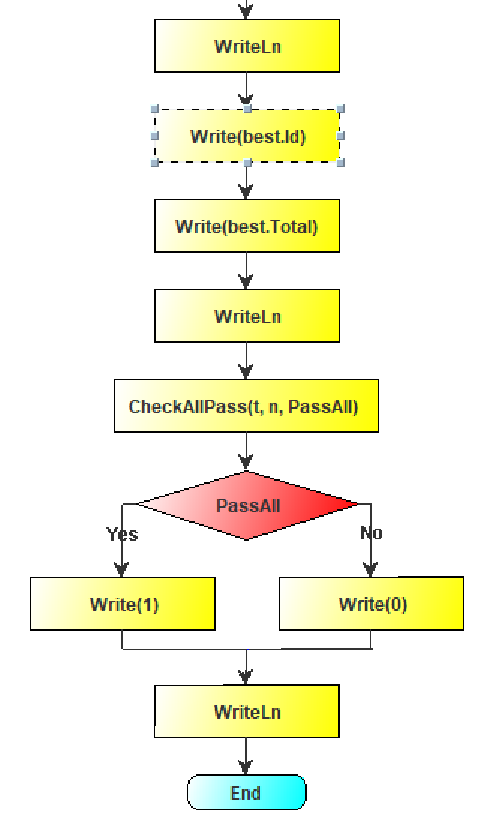
\includegraphics[width=\textwidth]{img/print_all2.png}
        \caption{PrintAll 流程图 (下半部分)}
        \label{fig:flow-printall2}
    \end{minipage}
    \vspace{0.2cm}
    \caption{PrintAll 过程的完整递归下降流程图展示}
    \label{fig:flow-printall}
\end{figure}

\section{实验心得与体会}

\begin{itemize}

\item \textbf{文法 → 代码的直接映射}
递归下降的方法调用链（\texttt{parseExpression → parseSimpleExpr → parseTerm
→ parseFactor}）与 BNF 层次结构一一对应——"读代码即读 BNF"。
乘除方法调用加减方法作为子过程，优先级编码直观无歧义。

\item \textbf{属性传递即方法签名}
方法参数 = 继承属性，返回值 = 综合属性，

例如\texttt{parseStatementSequence(ifStmt.getTrueBody())} 一行同时完成三件事：
声明归属容器（True 分支）、启动递归解析、语句节点自动回流——
信息流的自解释性远超 LR 语义动作。

\item \textbf{Flowchart 节点创建时机决定模型正确性。}
在解析方法入口处（如 \texttt{parseWhileStatement()} 开头）立即创建流程图节点，
而非解析结束后补建，确保语法分析与模型构造同步推进，不遗漏中间节点。

\item \textbf{EBNF 闭包 → while 循环的等价变换。}
花括号闭包 \texttt{\{AddOperator Term\}} 直接映射为 while 循环，无需显式
消除左递归或提取左公因子，保持了文法到代码的"零重写"桥梁。

\item \textbf{健壮性仰赖于异常处理。}
深层方法中的语法异常可能回滚调用栈、丢弃未完成节点。
工业场景需配合恐慌模式（Panic-mode）的同步集合恢复机制，才能实现多错误报告。

\end{itemize}


\end{document}
